              
% ****** Start of file apssamp.tex ******
%
%   This file is part of the APS files in the REVTeX 4.1 distribution.
%   Version 4.1r of REVTeX, August 2010
%
%   Copyright (c) 2009, 2010 The American Physical Society.
%
%   See the REVTeX 4 README file for restrictions and more information.
%
% TeX'ing this file requires that you have AMS-LaTeX 2.0 installed
% as well as the rest of the prerequisites for REVTeX 4.1
%
% See the REVTeX 4 README file
% It also requires running BibTeX. The commands are as follows:
%
%  1)  latex apssamp.tex
%  2)  bibtex apssamp
%  3)  latex apssamp.tex
%  4)  latex apssamp.tex
%
\documentclass[%
 reprint,
%superscriptaddress,
%groupedaddress,
%unsortedaddress,
%runinaddress,
%frontmatterverbose, 
%preprint,
%showpacs,preprintnumbers,
%nofootinbib,
%nobibnotes,
%bibnotes,
 amsmath,amssymb,
 aps,
%pra,
%prb,
%rmp,
%prstab,
%prstper,
%floatfix,
]{revtex4-1}

\usepackage{pgfplotstable}
\usepackage{array}
\usepackage{graphicx}% Include figure files
\usepackage{dcolumn}% Align table columns on decimal point
\usepackage{bm}% bold math
\usepackage{hyperref}% add hypertext capabilities
%\usepackage[mathlines]{lineno}% Enable numbering of text and display math
%\linenumbers\relax % Commence numbering lines

%\usepackage[showframe,%Uncomment any one of the following lines to test 
%%scale=0.7, marginratio={1:1, 2:3}, ignoreall,% default settings
%%text={7in,10in},centering,
%%margin=1.5in,
%%total={6.5in,8.75in}, top=1.2in, left=0.9in, includefoot,
%%height=10in,a5paper,hmargin={3cm,0.8in},
%]{geometry}
\bibliographystyle{plain}

%\graphicspath{{C:\Users\Nick\Documents\GitHub\FYS2150\lab1}}

\begin{document}

%\preprint{APS/123-QED}

\title{Lab Report: Length, Velocity and Acceleration}% Force line breaks with \\

\author{Nicholas Karlsen}
% \email{nichoka@student.matnat.uio.no}

\date{\today}% It is always \today, today,
             %  but any date may be explicitly specified

\begin{abstract}
  A study on different methods for determining the length, velocity and acceleration of different objects, and the errors involved in these methods.
\end{abstract}

\maketitle

%\tableofcontents

\section{\label{sec:intro}Introduction}

\section{\label{sec:theory}Theory}
  \subsection{Pendulum}
    \begin{equation}
      \label{eqn:period}
        T \approx 2\pi \sqrt{\frac{L}{g}}\enspace
    \end{equation}
    Where $T$ denotes the period of a pendulum, $L$ its length and $g$ the gravitational acceleration. The small angle approximation (Eqn. \ref{eqn:period})  is valid for angles $\theta \ll 1\, \textup{rad}$ with an error $\approx \pm 15 \, \textup{s}$ per day \cite{pend_wik}.
  \subsection{Errors}
    \begin{equation}
    \label{eqn:sigma}
      \sigma \approx \left(
      \frac{\sum x_i^2 - \frac{1}{n}(\sum x_i)^2}
      {n - 1}
      \right)^\frac{1}{2}
    \end{equation}
    
    \begin{equation}
      \label{eqn:sigma_m}
      \sigma_m \approx \left(
      \frac{\sum x_i^2 - \frac{1}{n}(\sum x_i)^2}
      {n(n - 1)}
      \right)^\frac{1}{2}
    \end{equation}

    Where $\sigma, \sigma_m$ denotes the standard deviation, and the standard deviation of the mean respectively of a set of $n$ values $x_i$. \cite{squires}.

    Any errors stated in a derived number will be calculated using the equations for combinations of errors found on page 29 in Squires \cite{squires}. Lastly, when using a linear fit on a set of linearly correlated data i used the expressions found on page 39 in Squires \cite{squires} to calculate the regression line, as well as its error.

\section{\label{sec:exp_proced}Experimental Procedure}
  \section{Measuring the lenght of a rod}
  \section{Measuring the period and height of the Foucault's pendulum}
  \section{Measuring the velocity of the lego-car}
  \section{Measuring the velocity of the RC-car}

\section{\label{sec:data} Results}
  \begin{table}
    \caption{Lenght of rods}
    \label{tab:lenrods}
    \begin{tabular}{rrrrrrrrr}
\hline
Ruler & Ruler & Ruler & Ruler & Laser & Laser & Laser & Laser & Vernier Calliper \\
   $l_a [cm]$ &  $\delta l_a$ [cm] &   $l_b$ [cm] &   $\delta l_b$ [cm] &   $l_a$ [cm] &   $\delta l_a$ [cm] & $l_b$ [cm] &   $\delta l_b$ [cm] & $l_{a, b}$ [mm] \\
\hline
           119.50 &              0.23 &           119.60 &              0.23 &           120.50 &              0.20 &           120.60 &              0.20 &                         1.25 $\pm 0.05$ \\
           119.50 &              - &           119.70 &              - &           119.60 &              0.20 &           119.80 &              0.20 &                         - \\
           119.45 &              0.37 &           119.60 &              0.37 &           119.50 &              0.20 &           119.70 &              0.20 &                         1.40 $\pm 0.05$\\
           119.40 &              - &           119.50 &              - &           119.40 &              0.20 &           119.60 &              0.20 &                         - \\
           119.43 &              0.40 &           119.55 &              0.40 &           119.40 &              0.20 &           119.60 &              0.20 &                         1.20 $\pm $0.6\\
           119.40 &              0.20 &           119.60 &              0.20 &           119.68 &              0.20 &           119.72 &              0.20 &                         1.80 $\pm $0.05\\
           119.40 &              0.27 &           119.50 &              0.27 &           119.90 &              0.20 &           119.70 &              0.20 &                         0.00 $\pm 0.05$\\
           119.45 &              0.35 &           119.65 &              0.35 &           130.60 &              0.20 &           130.20 &              0.20 &                         1.80 $\pm $0.05\\
           119.40 &              - &           119.60 &              - &           119.40 &              0.22 &           119.50 &              0.22 &                         - \\
           119.43 &              0.31 &           119.55 &              0.31 &             - &              - &             - &              - &                         1.50 $\pm 0.05$\\
\hline
\end{tabular}

  \end{table}

  \begin{table}
    \caption{Uncertainty in Length measurement}
    \label{tab:uncert}
    \begin{tabular}{| l | l | l |}
\hline
 & $x$ & $\delta x$ \\
\hline
$l_a$                 & $119.5cm$ &    \\             
$l_b$                 & $119.6cm$ &    \\        
$dl_s$                &     & $1.4mm$   \\             
$\sqrt{n}\cdot dl_l$  &     & $0.5\sqrt{5}mm$   \\                  
$dl_m$                &     & $1.4mm$   \\                  
$\alpha l_a (T-25C)$  & $-0.156cm$ & $\sim 10^{-6}$   \\ 
\hline                

\end{tabular}

\begin{tabular}{| l | l | l |}
\hline
& $\sum x_i$ & $\sqrt {\sum \sigma x_i^2 }$ \\
\hline
$\sum l_a$ & 119.48cm & 2.27 \\
$\sum l_b$ & 119.58cm & 2.27 \\
\hline   
\end{tabular}
  \end{table}
  
  \begin{table}
    \caption{Period of pendulum}
    \label{tab:pendel}
    \begin{tabular}{rrrr}
\hline
   T [s]\\
\hline
    7.30\\ 7.72\\ 7.57\\ 7.43\\ 7.73\\ 7.27\\ 7.68\\ 7.60\\ 7.34\\ 7.75\\
    7.06\\ 7.32\\ 7.55\\ 7.29\\ 7.08\\ 7.82\\ 7.78\\ 7.44\\ 7.68\\ 7.46\\
\hline
\end{tabular}

  \end{table}
  \begin{figure}[h!]
    \center
    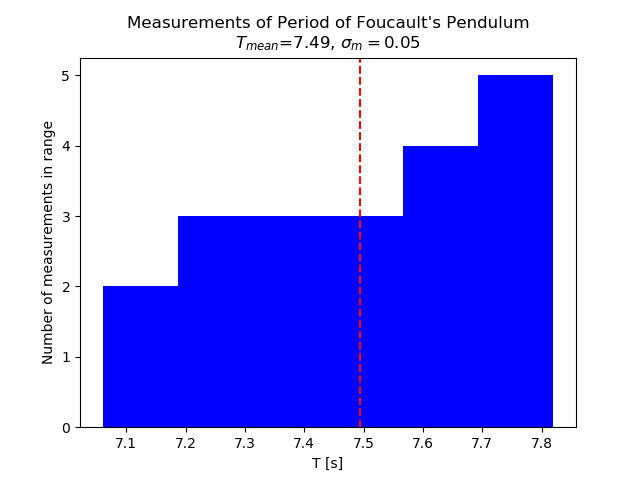
\includegraphics[scale=0.5]{scripts/figs/period.png}
    \caption{Measurements of the Period of the Focault's Pendulum in the entrance hall at the Institute of Physics, UiO.}
    \label{fig:pendel}
  \end{figure}


\section{\label{sec:disc}Discussion}
\section{\label{sec:conc}Conclusion}


    \bibliography{rapport2_ref}
\end{document}
%
% ****** End of file apssamp.tex ******
              